\documentclass[conference]{IEEEtran}
\IEEEoverridecommandlockouts
\usepackage[utf8]{inputenc}
\usepackage[T1]{fontenc}
\usepackage[brazil]{babel}
\usepackage{cite}
\usepackage{amsmath}
\usepackage{graphicx}
\usepackage{booktabs}
\usepackage{url}
\usepackage[hidelinks]{hyperref}

% gerado por src/m06_figuras_tabelas.py - não editar
\newcommand{\nInstancias}{11.470}
\newcommand{\nAtributos}{21}
\newcommand{\pctAnormal}{42,7}
\newcommand{\pctNormal}{57,3}
\newcommand{\melhorNome}{Random Forest}
\newcommand{\tCincoDois}{3,44}
\newcommand{\pCincoDois}{0,018}
\newcommand{\erroLogreg}{26,3}
\newcommand{\erroMelhor}{25,6}
\newcommand{\aucDummy}{0,500}
\newcommand{\aucPrDummy}{0,427}
\newcommand{\recallDummy}{0,000}
\newcommand{\fUmDummy}{0,000}
\newcommand{\acBalDummy}{0,500}
\newcommand{\acurDummy}{0,573}
\newcommand{\especDummy}{1,000}
\newcommand{\precDummy}{0,000}
\newcommand{\aucDpDummy}{0,000}
\newcommand{\aucLogreg}{0,787}
\newcommand{\aucPrLogreg}{0,759}
\newcommand{\recallLogreg}{0,587}
\newcommand{\fUmLogreg}{0,656}
\newcommand{\acBalLogreg}{0,719}
\newcommand{\acurLogreg}{0,738}
\newcommand{\especLogreg}{0,850}
\newcommand{\precLogreg}{0,745}
\newcommand{\aucDpLogreg}{0,012}
\newcommand{\aucArvore}{0,774}
\newcommand{\aucPrArvore}{0,734}
\newcommand{\recallArvore}{0,572}
\newcommand{\fUmArvore}{0,643}
\newcommand{\acBalArvore}{0,709}
\newcommand{\acurArvore}{0,729}
\newcommand{\especArvore}{0,846}
\newcommand{\precArvore}{0,735}
\newcommand{\aucDpArvore}{0,018}
\newcommand{\aucRf}{0,802}
\newcommand{\aucPrRf}{0,770}
\newcommand{\recallRf}{0,590}
\newcommand{\fUmRf}{0,665}
\newcommand{\acBalRf}{0,726}
\newcommand{\acurRf}{0,746}
\newcommand{\especRf}{0,862}
\newcommand{\precRf}{0,761}
\newcommand{\aucDpRf}{0,015}
\newcommand{\aucGb}{0,800}
\newcommand{\aucPrGb}{0,769}
\newcommand{\recallGb}{0,578}
\newcommand{\fUmGb}{0,659}
\newcommand{\acBalGb}{0,724}
\newcommand{\acurGb}{0,745}
\newcommand{\especGb}{0,869}
\newcommand{\precGb}{0,767}
\newcommand{\aucDpGb}{0,015}
\newcommand{\aucMelhor}{0,802}
\newcommand{\aucPrMelhor}{0,770}
\newcommand{\recallMelhor}{0,590}
\newcommand{\fUmMelhor}{0,665}
\newcommand{\acBalMelhor}{0,726}
\newcommand{\acurMelhor}{0,746}
\newcommand{\especMelhor}{0,862}
\newcommand{\precMelhor}{0,761}
\newcommand{\aucDpMelhor}{0,015}
\newcommand{\aucComSoproLogreg}{0,945}
\newcommand{\recallComSoproLogreg}{0,871}
\newcommand{\aucRestritoLogreg}{0,697}
\newcommand{\recallRestritoLogreg}{0,412}
\newcommand{\recallPesosLogreg}{0,638}
\newcommand{\especPesosLogreg}{0,811}
\newcommand{\fUmPesosLogreg}{0,674}
\newcommand{\aucPesosLogreg}{0,787}
\newcommand{\recallSmoteLogreg}{0,635}
\newcommand{\especSmoteLogreg}{0,816}
\newcommand{\fUmSmoteLogreg}{0,675}
\newcommand{\aucSmoteLogreg}{0,787}
\newcommand{\recallSubLogreg}{0,638}
\newcommand{\especSubLogreg}{0,812}
\newcommand{\fUmSubLogreg}{0,675}
\newcommand{\aucSubLogreg}{0,787}
\newcommand{\aucAgrupadoLogreg}{0,788}
\newcommand{\recallAgrupadoLogreg}{0,587}
\newcommand{\vpLogreg}{2.873}
\newcommand{\fnLogreg}{2.021}
\newcommand{\fpLogreg}{986}
\newcommand{\vnLogreg}{5.590}
\newcommand{\aucComSoproMelhor}{0,953}
\newcommand{\recallComSoproMelhor}{0,875}
\newcommand{\aucRestritoMelhor}{0,722}
\newcommand{\recallRestritoMelhor}{0,450}
\newcommand{\recallPesosMelhor}{0,642}
\newcommand{\especPesosMelhor}{0,821}
\newcommand{\fUmPesosMelhor}{0,682}
\newcommand{\aucPesosMelhor}{0,802}
\newcommand{\recallSmoteMelhor}{0,622}
\newcommand{\especSmoteMelhor}{0,836}
\newcommand{\fUmSmoteMelhor}{0,675}
\newcommand{\aucSmoteMelhor}{0,802}
\newcommand{\recallSubMelhor}{0,653}
\newcommand{\especSubMelhor}{0,809}
\newcommand{\fUmSubMelhor}{0,684}
\newcommand{\aucSubMelhor}{0,801}
\newcommand{\aucAgrupadoMelhor}{0,801}
\newcommand{\recallAgrupadoMelhor}{0,591}
\newcommand{\vpMelhor}{2.886}
\newcommand{\fnMelhor}{2.008}
\newcommand{\fpMelhor}{905}
\newcommand{\vnMelhor}{5.671}
\newcommand{\fnLimiarCinquenta}{2.008}
\newcommand{\fpLimiarCinquenta}{905}
\newcommand{\recallLimiarCinquenta}{0,590}
\newcommand{\precLimiarCinquenta}{0,761}
\newcommand{\especLimiarCinquenta}{0,862}
\newcommand{\fnLimiarTrinta}{853}
\newcommand{\fpLimiarTrinta}{2.814}
\newcommand{\recallLimiarTrinta}{0,826}
\newcommand{\precLimiarTrinta}{0,589}
\newcommand{\especLimiarTrinta}{0,572}
\newcommand{\fnLimiarQuarenta}{1.528}
\newcommand{\fpLimiarQuarenta}{1.487}
\newcommand{\recallLimiarQuarenta}{0,688}
\newcommand{\precLimiarQuarenta}{0,694}
\newcommand{\especLimiarQuarenta}{0,774}
\newcommand{\impUm}{Motivo 2}
\newcommand{\impValorUm}{0,075}
\newcommand{\impDois}{Motivo 1}
\newcommand{\impValorDois}{0,038}
\newcommand{\impTres}{B2}
\newcommand{\impValorTres}{0,033}
\newcommand{\impQuatro}{FC}
\newcommand{\impValorQuatro}{0,023}
\newcommand{\impCinco}{HDA ausente}
\newcommand{\impValorCinco}{0,013}
\newcommand{\pctFnMelhor}{41,0}
\newcommand{\reducaoFnTrinta}{58}
\newcommand{\idadeVp}{1,1}
\newcommand{\fcVp}{100}
\newcommand{\parecerVp}{5}
\newcommand{\suspeitaVp}{66}
\newcommand{\idadeFn}{4,6}
\newcommand{\fcFn}{92}
\newcommand{\parecerFn}{59}
\newcommand{\suspeitaFn}{25}
\newcommand{\idadeFp}{1,3}
\newcommand{\fcFp}{100}
\newcommand{\parecerFp}{5}
\newcommand{\suspeitaFp}{63}
\newcommand{\idadeVn}{5,3}
\newcommand{\fcVn}{88}
\newcommand{\parecerVn}{67}
\newcommand{\suspeitaVn}{20}
\newcommand{\soproSistolico}{95,9}
\newcommand{\soproAusente}{10,1}
\newcommand{\vSopro}{0,84}
\newcommand{\vBDois}{0,24}
\newcommand{\vMotivoDois}{0,46}
\newcommand{\rcBDoisNormal}{0,18}
\newcommand{\rcMotivoSopro}{3,72}
\newcommand{\rcBDoisHiper}{2,79}
\newcommand{\rcHdaAusente}{0,48}
\newcommand{\ganhoSopro}{0,15}
\newcommand{\pctAusentePa}{55,5}
\newcommand{\pctAusentePpa}{81,9}
\newcommand{\tempoMin}{49}
\newcommand{\cLogreg}{0,1}
\newcommand{\paramsMelhor}{max\_depth = None, max\_features = sqrt, min\_samples\_leaf = 5}

\renewcommand{\IEEEkeywordsname}{Palavras-chave}

% ---------------------------------------------------------------- preencher antes da entrega
\newcommand{\repositorio}{\url{https://github.com/Caio424/Trabalho_DataMining}}
\newcommand{\autores}{Caio Moreira Bovo, Pedro Henrique Santana, Rafael Alencar Delfino, Yuri Resende Camargo}
\newcommand{\afiliacao}{Mineração de Dados -- Grupo~10\\Universidade Federal de Goiás (UFG)}
% ---------------------------------------------------------------------------------------------

\begin{document}

\title{Triagem de Patologia Cardíaca Pediátrica com Dados de Encaminhamento: Comparação de Classificadores e Controle de Vazamento de Dados%
\thanks{Código, resultados e instruções de reprodução (\texttt{random\_state} = 42): \repositorio.}}

\author{\IEEEauthorblockN{\autores}
\IEEEauthorblockA{\afiliacao}}

\maketitle

\begin{abstract}
Este trabalho investiga a triagem automática de patologia cardíaca pediátrica (0 a 19 anos) a partir dos dados de encaminhamento a um serviço especializado. Sobre o conjunto UCMF, com \nInstancias{} pacientes após a limpeza, formulamos uma tarefa de classificação binária (Normal $\times$ Anormal) e excluímos o atributo Sopro, que caracteriza vazamento de dados. Comparamos um baseline de Regressão Logística com Árvore de Decisão, Random Forest e Gradient Boosting, em validação cruzada aninhada estratificada, com todo o pré-processamento ajustado apenas no treino. A \melhorNome{} obteve AUC-ROC de \aucMelhor{}, contra \aucLogreg{} do baseline, e reduziu a taxa de erro de \erroLogreg\% para \erroMelhor\%: diferença pequena, mas significativa pelos testes 5$\times$2cv ($p$~=~\pCincoDois{} e \pFCincoDois). Com o Sopro, a AUC chegaria a \aucComSoproMelhor{}, o que mostra o tamanho do vazamento. Os motivos de encaminhamento são os atributos mais informativos, e o modelo não detecta \pctFnMelhor\% dos casos anormais no limiar padrão.
\end{abstract}

\begin{IEEEkeywords}
classificação, cardiologia pediátrica, vazamento de dados, validação cruzada aninhada, aprendizado de máquina
\end{IEEEkeywords}

% =============================================================================================
\section{Introdução}

Grande parte das crianças encaminhadas a um ambulatório de cardiologia pediátrica não tem doença cardíaca: os encaminhamentos por sopro inocente, pareceres pré-operatórios e check-ups ocupam a agenda de especialistas escassos. Uma ferramenta que estime, \emph{antes} da consulta, a probabilidade de patologia ajudaria a priorizar quem deve ser atendido primeiro.

O objetivo deste trabalho é uma tarefa de \textbf{classificação binária}: prever se o paciente terá diagnóstico \emph{Normal} ou \emph{Anormal} a partir de dados demográficos, antropométricos, sinais vitais, histórico e motivos de encaminhamento. Como a classe de interesse é a Anormal, o erro mais grave é o falso negativo: uma criança doente classificada como saudável.

A contribuição é metodológica e prática: (i) identificamos e medimos o vazamento de dados causado pelo atributo Sopro; (ii) avaliamos quatro classificadores com um protocolo sem vazamento (validação aninhada e pré-processamento dentro do pipeline), com teste estatístico de comparação; e (iii) interpretamos os erros e os atributos mais relevantes no contexto clínico.

% =============================================================================================
\section{Dados e Análise Exploratória}

O conjunto UCMF, fornecido no estudo de caso da disciplina, reúne atendimentos de cardiologia pediátrica, concentrados entre 2003 e 2010, de pacientes de 0 a 19 anos. Após a limpeza descrita na Seção~\ref{sec:metodologia}, restaram \nInstancias{} instâncias e \nAtributos{} atributos de entrada (Tabela~\ref{tab:dados}). A variável-alvo indica ausência ou presença de patologia cardíaca, com desbalanceamento leve: \pctNormal\% Normal e \pctAnormal\% Anormal.

\begin{table}[!t]
\caption{Características do conjunto após a limpeza}
\label{tab:dados}
\centering\footnotesize
\begin{tabular}{@{}lr@{}}
\toprule
Característica & Valor \\
\midrule
Instâncias (bruto $\rightarrow$ limpo) & 12.873 $\rightarrow$ 11.470 \\
Atributos de entrada (antes da codificação) & 21 \\
Classe Normal / Anormal & 57,3\% / 42,7\% \\
Ausentes: Idade & 6,7\% \\
Ausentes: IMC & 33,9\% \\
Ausentes: Pressão arterial (PAS/PAD) & 55,5\% \\
Ausentes: Frequência cardíaca & 6,2\% \\
Ausentes: Motivo 2 & 22,1\% \\
Ausentes: PPA & 81,9\% \\
Ausentes: HDA (histórico) & 25,9\% \\
\bottomrule
\end{tabular}

\end{table}

As ausências são o principal problema de qualidade. A pressão arterial falta em \pctAusentePa\% dos registros, e a classificação de hipertensão (PPA) em \pctAusentePpa\%, porque a planilha de origem registrava erro de fórmula ou ``Não Calculado''. A ausência não é aleatória: a pressão raramente é medida em lactentes. Por isso, em vez de descartar as variáveis, mantivemos indicadores de ausência.

\textbf{Vazamento de dados.} A análise bivariada da etapa anterior (A1) mostrou que o Sopro tem associação muito acima dos demais atributos com o alvo (V de Cramér de \vSopro{}, contra \vMotivoDois{} do segundo colocado; Fig.~\ref{fig:leakage}). Entre os pacientes com sopro sistólico, \soproSistolico\% são Anormais; sem sopro, apenas \soproAusente\%. O Sopro é um achado do exame físico feito pelo próprio cardiologista, na mesma consulta que define o diagnóstico. Um modelo que o usa estaria ``lendo'' a conclusão do médico, e não fazendo triagem antes da consulta, o que caracteriza vazamento de dados~\cite{kaufman2012}. O atributo foi \textbf{excluído} da análise principal; mantivemos um cenário com ele apenas para medir o tamanho do efeito.

\begin{figure}[!t]
\centering
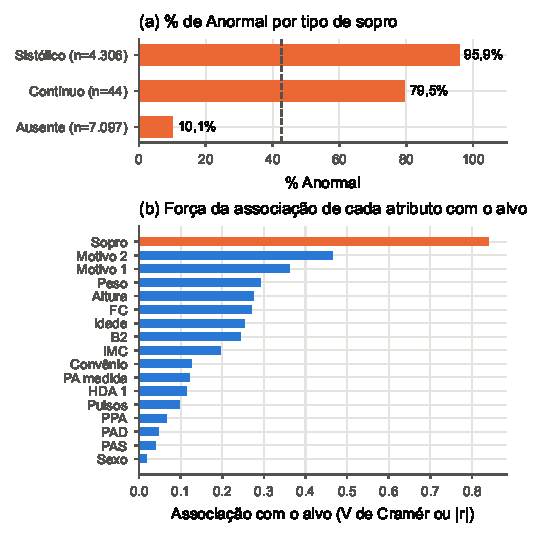
\includegraphics[width=\columnwidth]{figuras/fig1_leakage.pdf}
\caption{Evidência de vazamento. (a) Proporção de Anormais por tipo de sopro; a linha tracejada é a proporção geral. (b) Associação de cada atributo com o alvo na análise bivariada da A1; o Sopro destoa de todos os demais.}
\label{fig:leakage}
\end{figure}

% =============================================================================================
\section{Metodologia}
\label{sec:metodologia}

\textbf{Limpeza.} Partimos do arquivo bruto (\nBruto{} registros) e aplicamos as 34 regras da A1: remoção de duplicatas e de registros sem rótulo, recálculo da idade a partir das datas e do IMC a partir de peso e altura, e anulação de valores fisiologicamente impossíveis segundo faixas amplas de plausibilidade baseadas na OMS~\cite{oms2006}, em Fleming~\textit{et~al.}~\cite{fleming2011} e em Flynn~\textit{et~al.}~\cite{flynn2017}. Nenhum valor é imputado nessa etapa.

\textbf{Atributos e transformações.} Usamos idade, IMC, pressão sistólica e diastólica, frequência cardíaca (FC), sexo, convênio, pulsos, segunda bulha (B2), os dois motivos de encaminhamento, a PPA ordinal e sete indicadores de sintoma derivados do histórico (HDA). Identificador, datas, peso e altura foram removidos, pois a informação está na idade e no IMC. Todas as transformações que aprendem com os dados ficam dentro de um \emph{pipeline} e são reajustadas em cada partição de treino: logaritmo nas variáveis assimétricas (IMC, PAS, FC), imputação pela mediana com indicador de ausência, padronização (z-score) e codificação one-hot, com categorias raras ($n<30$) agrupadas. Assim, nenhuma estatística do conjunto de teste participa do ajuste.

\textbf{Protocolo de validação.} Com \nInstancias{} instâncias, seguimos a recomendação de validação cruzada estratificada em 10 partições~\cite{kohavi1995}, na forma \emph{aninhada}: em cada partição externa, uma validação interna estratificada de 5 partições escolhe os hiperparâmetros por busca em grade (critério AUC-ROC), e o modelo final é avaliado na partição externa, nunca vista. Cada instância é avaliada exatamente uma vez. Como a base não tem identificador de paciente, repetimos a avaliação com partição agrupada por data de nascimento e sexo, para verificar se possíveis retornos do mesmo paciente vazavam entre treino e teste. Nos experimentos de desbalanceamento e de partição agrupada, para reduzir o custo, os hiperparâmetros foram fixados nos mais escolhidos pela busca aninhada. Como essa escolha viu as mesmas partições, esses experimentos são comparados apenas entre si, a partir da linha \emph{sem tratamento} da Tabela~\ref{tab:ablacao}, e não com a Tabela~\ref{tab:modelos}.

\textbf{Métricas.} Relatamos média e desvio-padrão, nos 10 folds, de acurácia, acurácia balanceada, precisão, recall (sensibilidade), especificidade, F1, AUC-ROC e AUC-PR. Para triagem, o recall da classe Anormal é a métrica mais importante; a AUC-ROC mede a capacidade de ordenar pacientes por risco independentemente do limiar.

\textbf{Algoritmos.} A Regressão Logística é o baseline simples (C $\in \{0{,}01; 0{,}1; 1; 10\}$). Os modelos complexos são a Árvore de Decisão (profundidade e tamanho mínimo da folha), a Random Forest~\cite{breiman2001} (300 árvores; profundidade, tamanho da folha e fração de atributos) e o Gradient Boosting baseado em histogramas~\cite{friedman2001,ke2017} (taxa de aprendizado, profundidade e regularização L2). Uma classe majoritária serve de piso de referência. Implementação em scikit-learn~\cite{pedregosa2011} e imbalanced-learn~\cite{lemaitre2017}.

\textbf{Desbalanceamento.} Para o baseline e o melhor modelo complexo, comparamos sem tratamento, pesos por classe, SMOTE~\cite{chawla2002} e subamostragem aleatória. A reamostragem ocorre somente no treino, dentro do pipeline. Também analisamos o efeito do limiar de decisão.

\textbf{Comparação estatística.} Comparamos o baseline e o melhor modelo complexo com o teste t 5$\times$2cv de Dietterich~\cite{dietterich1998}, sobre a taxa de erro, com $\alpha = 0{,}05$ e 5 graus de liberdade; em cada uma das 10 execuções, os hiperparâmetros são reajustados no treino. Como a estatística t usa apenas a diferença da primeira execução, reportamos também o teste F combinado de Alpaydin~\cite{alpaydin1999}, que usa as 10 diferenças. A importância dos atributos foi medida por permutação nos folds de teste (queda da AUC-ROC), sobre as colunas originais. O experimento completo levou cerca de \tempoMin{} minutos.

% =============================================================================================
\section{Resultados e Discussão}

\begin{table*}[!t]
\caption{Desempenho na validação cruzada aninhada (média e desvio-padrão em 10 folds; cenário sem Sopro; limiar 0,5). Em negrito, o melhor valor entre os modelos treinados}
\label{tab:modelos}
\centering\footnotesize
\begin{tabular}{@{}lcccccccc@{}}
\toprule
Modelo & Acur. & Ac. bal. & Prec. & Recall & Espec. & F1 & AUC-ROC & AUC-PR \\
\midrule
Classe majoritária & 0,573 (0,000) & 0,500 (0,000) & 0,000 (0,000) & 0,000 (0,000) & 1,000 (0,000) & 0,000 (0,000) & 0,500 (0,000) & 0,427 (0,000) \\
Regressão Logística & 0,738 (0,011) & 0,719 (0,012) & 0,745 (0,018) & 0,587 (0,018) & 0,850 (0,012) & 0,656 (0,016) & 0,787 (0,012) & 0,759 (0,018) \\
Árvore de Decisão & 0,729 (0,018) & 0,709 (0,019) & 0,735 (0,027) & 0,572 (0,028) & 0,846 (0,018) & 0,643 (0,026) & 0,774 (0,018) & 0,734 (0,024) \\
Random Forest & \textbf{0,746 (0,014)} & \textbf{0,726 (0,014)} & \textbf{0,761 (0,021)} & 0,590 (0,017) & \textbf{0,862 (0,013)} & 0,665 (0,018) & \textbf{0,802 (0,015)} & 0,770 (0,021) \\
Gradient Boosting & 0,745 (0,014) & 0,726 (0,013) & 0,758 (0,026) & \textbf{0,592 (0,015)} & 0,859 (0,019) & \textbf{0,665 (0,016)} & 0,801 (0,015) & \textbf{0,771 (0,022)} \\
\bottomrule
\end{tabular}

\end{table*}

\textbf{Comparação dos modelos.} A Tabela~\ref{tab:modelos} e a Fig.~\ref{fig:curvas} mostram que todos os modelos superam com folga o piso da classe majoritária, mas ficam próximos entre si. A \melhorNome{} obteve a maior AUC-ROC (\aucMelhor{} $\pm$ \aucDpMelhor), seguida de \ordemDemais. As curvas ROC e Precisão--Recall praticamente se sobrepõem. O teste t 5$\times$2cv indica que a vantagem da \melhorNome{} sobre o baseline, medida pela taxa de erro, é estatisticamente significativa ($t$~=~\tCincoDois, $p$~=~\pCincoDois); o teste F combinado, que não depende de uma única execução, confirma ($F$~=~\fCincoDois, $p$~=~\pFCincoDois). O tamanho do efeito, porém, é modesto: a taxa de erro cai de \erroLogreg\% para \erroMelhor\%. Em outras palavras, o ganho é consistente entre partições, porém pequeno; a Regressão Logística, mais simples e interpretável, é uma alternativa quase equivalente. Os hiperparâmetros mais escolhidos foram C = \cLogreg{} na Regressão Logística e \paramsMelhor{} na \melhorNome. Os desvios-padrão baixos indicam estimativas estáveis entre as partições.

\begin{figure*}[!t]
\centering
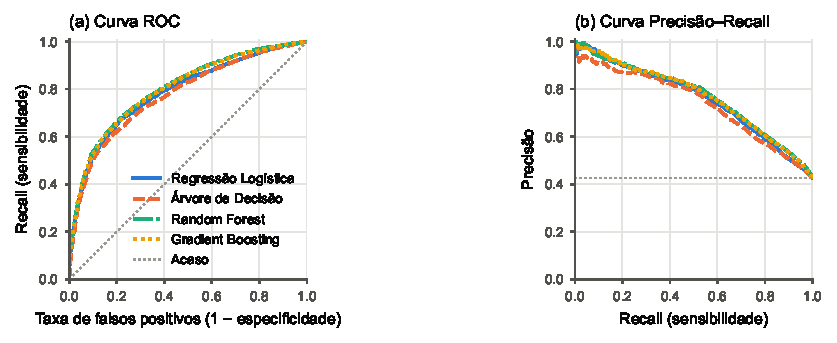
\includegraphics[width=0.70\textwidth]{figuras/fig2_curvas.pdf}
\caption{Curvas ROC e Precisão--Recall com as previsões fora da amostra dos 10 folds externos (cenário sem Sopro). A linha pontilhada indica o desempenho ao acaso.}
\label{fig:curvas}
\end{figure*}

\textbf{Tamanho do vazamento e dependência dos atributos.} A Tabela~\ref{tab:ablacao} mostra que, com o Sopro, a AUC subiria para \aucComSoproLogreg{} (Regressão Logística) e \aucComSoproMelhor{} (\melhorNome), e o recall para cerca de \recallComSoproMelhor. Esse salto de \ganhoSopro{} na AUC é o desempenho ``emprestado'' do diagnóstico médico, que não estaria disponível no momento da triagem. Os motivos de encaminhamento são os atributos individualmente mais importantes: sem eles, a AUC cai para \aucRestritoLogreg{} e \aucRestritoMelhor{}, mas cerca de \pctSinalSemMotivos\% da discriminação acima do acaso permanece. A B2, outro achado de ausculta, pesa bem menos: sem ela, a AUC fica em \aucSemBDoisLogreg{} e \aucSemBDoisMelhor{}.

\begin{table}[!t]
\caption{Análise de ablação: atributos, desbalanceamento e validação agrupada (médias em 10 folds)}
\label{tab:ablacao}
\centering\scriptsize\setlength{\tabcolsep}{3.5pt}
\begin{tabular}{@{}lcccccc@{}}
\toprule
 & \multicolumn{3}{c}{Regressão Logística} & \multicolumn{3}{c}{Random Forest} \\
\cmidrule(lr){2-4}\cmidrule(l){5-7}
Configuração & AUC & Rec. & F1 & AUC & Rec. & F1 \\
\midrule
\multicolumn{7}{@{}l}{\textit{Atributos}} \\
Com Sopro (vazamento) & 0,945 & 0,871 & 0,910 & 0,953 & 0,875 & 0,912 \\
Sem Sopro (principal) & 0,787 & 0,587 & 0,656 & 0,802 & 0,590 & 0,665 \\
Sem Sopro e Motivos & 0,697 & 0,412 & 0,507 & 0,722 & 0,450 & 0,541 \\
\midrule
\multicolumn{7}{@{}l}{\textit{Desbalanceamento}} \\
Sem tratamento & 0,787 & 0,587 & 0,656 & 0,802 & 0,591 & 0,665 \\
Pesos por classe & 0,787 & 0,638 & 0,674 & 0,802 & 0,642 & 0,682 \\
SMOTE & 0,787 & 0,635 & 0,675 & 0,802 & 0,622 & 0,675 \\
Subamostragem & 0,787 & 0,638 & 0,675 & 0,801 & 0,653 & 0,684 \\
\midrule
\multicolumn{7}{@{}l}{\textit{Validação}} \\
Agrupada por paciente & 0,788 & 0,587 & 0,657 & 0,801 & 0,591 & 0,664 \\
\bottomrule
\end{tabular}

\end{table}

\textbf{Desbalanceamento e limiar.} Como o desbalanceamento é leve, nenhuma estratégia altera a AUC: a ordenação dos pacientes por risco é a mesma. O que muda é o ponto de corte efetivo. Na \melhorNome, partindo da linha sem tratamento (recall \recallNenhumMelhor, especificidade \especNenhumMelhor), os pesos por classe elevam o recall para \recallPesosMelhor{} e a subamostragem para \recallSubMelhor{}, com queda da especificidade para \especPesosMelhor{} e \especSubMelhor{}. O ajuste direto do limiar é mais controlável: nas previsões fora da amostra, baixar o limiar de 0,5 para 0,3 reduz os doentes não detectados de \fnLimiarCinquenta{} para \fnLimiarTrinta{} (\reducaoFnTrinta\% a menos, recall \recallLimiarTrinta), ao custo de aumentar os falsos alarmes de \fpLimiarCinquenta{} para \fpLimiarTrinta{} (precisão \precLimiarTrinta). Em triagem, em que o falso negativo é o erro caro, um limiar mais baixo é preferível. A escolha exata, porém, é uma decisão clínica sobre a capacidade de atendimento, e não um parâmetro estatístico.

\textbf{Pacientes repetidos.} Com a partição agrupada, a AUC foi \aucAgrupadoLogreg{} e \aucAgrupadoMelhor{}, igual à da partição comum (Tabela~\ref{tab:ablacao}). Não há indício de vazamento por retorno do mesmo paciente.

\begin{figure*}[!t]
\centering
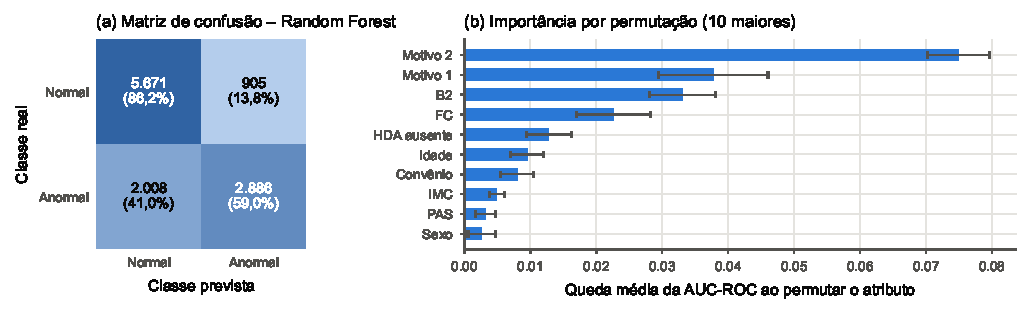
\includegraphics[width=0.84\textwidth]{figuras/fig3_erros_importancia.pdf}
\caption{\melhorNome{} no cenário sem Sopro. (a) Matriz de confusão das previsões fora da amostra, com o percentual em relação à classe real. (b) Queda média da AUC-ROC quando cada atributo é embaralhado no fold de teste; as barras indicam o desvio-padrão entre os folds.}
\label{fig:erros}
\end{figure*}

\textbf{Análise dos erros.} No limiar padrão, a \melhorNome{} classifica corretamente \vnMelhor{} Normais e \vpMelhor{} Anormais, mas deixa passar \fnMelhor{} pacientes doentes (\pctFnMelhor\% dos Anormais; Fig.~\ref{fig:erros}a). O perfil desses erros é revelador. Os verdadeiros positivos são, em geral, lactentes (idade mediana de \idadeVp{} ano), encaminhados por suspeita de cardiopatia (\suspeitaVp\%). Os falsos negativos são crianças mais velhas (mediana de \idadeFn{} anos), encaminhadas majoritariamente para parecer cardiológico (\parecerFn\%), um perfil indistinguível do dos verdadeiros negativos (\idadeVn{} anos; \parecerVn\% de parecer). Os falsos positivos são o espelho: lactentes com suspeita que se revelaram normais. O modelo aprendeu, portanto, o padrão ``bebê com suspeita'', e falha nos casos em que a doença aparece num encaminhamento de rotina.

\textbf{Atributos relevantes.} Pela importância por permutação (Fig.~\ref{fig:erros}b), os atributos mais relevantes são \impUm, \impDois, \impTres{} e \impQuatro. Os coeficientes da Regressão Logística apontam o mesmo sentido clínico. Como o modelo tem regularização L2 e codificação completa das categorias, $\exp(\beta)$ é uma razão de chances penalizada, indicativa do sentido e não da magnitude exata: o encaminhamento por sopro (\rcMotivoSopro) e a B2 hiperfonética (\rcBDoisHiper) aumentam a chance de patologia, e a B2 normal a reduz (\rcBDoisNormal). A FC mediana é maior entre os verdadeiros positivos do que entre os verdadeiros negativos (\fcVp{} contra \fcVn{} bpm), o que é coerente com a maior proporção de lactentes no primeiro grupo. A B2, assim como o Sopro, é um achado de ausculta. Ela foi mantida porque sua associação com o alvo é bem menor (V de \vBDois{}, contra \vSopro{} do Sopro) e porque removê-la custa pouco (AUC de \aucSemBDoisMelhor{}); para uma triagem estritamente anterior à consulta, o modelo sem B2 é a versão recomendada.

% =============================================================================================
\section{Conclusão}

Formulamos a triagem de patologia cardíaca pediátrica como classificação binária e mostramos que, sem o atributo de vazamento, os dados de encaminhamento permitem discriminar moderadamente os pacientes (AUC-ROC de \aucMelhor{} com \melhorNome). O ganho sobre a Regressão Logística é significativo, mas pequeno. Com ajuste do limiar, o modelo pode servir como apoio à priorização de agenda, mas não como substituto da avaliação clínica: mesmo com limiar reduzido, uma fração relevante dos doentes não é detectada.

As principais \textbf{limitações} são: (i) dados de um único serviço, concentrados entre 2003 e 2010, o que limita a generalização; (ii) a pressão arterial e a PPA têm muitas ausências; (iii) os motivos de encaminhamento refletem a suspeita de outro médico, e a B2 é um achado de exame, ainda que de peso pequeno; (iv) não há identificador real de paciente, e o agrupamento por data de nascimento e sexo é uma aproximação; (v) a validação é aleatória, e não temporal. Como \textbf{trabalhos futuros}, sugerimos validar o modelo em dados de outro período ou serviço, calibrar as probabilidades e definir o limiar com a equipe clínica a partir do custo de cada erro.

\section*{Declaração de uso de IA generativa}
O assistente Claude (Anthropic), por meio da ferramenta Claude Code, foi usado para apoiar a implementação do código em Python (pipeline, experimentos, testes e figuras), organizar o protocolo experimental a partir do material da disciplina e redigir uma primeira versão deste texto. Os integrantes revisaram o código, conferiram os resultados e são responsáveis pelo conteúdo final.

\bibliographystyle{IEEEtran}
\bibliography{refs}

\end{document}
